\documentclass[12pt]{article}
\usepackage[utf8]{inputenc}
\usepackage{upquote}
\usepackage[margin=1in]{geometry} 
\usepackage{amsmath,amsthm,amssymb}
\usepackage{graphicx}
\usepackage{listings}
\newenvironment{statement}[2][Statement]{\begin{trivlist}
\item[\hskip \labelsep {\bfseries #1}\hskip \labelsep {\bfseries #2.}]}{\end{trivlist}}
\usepackage{xcolor}




\title{Assignment 1}


\author{Author \\
  Wanjing Hu / fng685@alumni.ku.dk  \\
  Zhigao Yan / sxd343@alumni.ku.dk  \\
  Wanjing Hu / fng685@alumni.ku.dk  \\
  Wanjing Hu / fng685@alumni.ku.dk  \\
} 
 

\begin{document}
\maketitle


\section{26.1-1}
%wanjing
\textbf{Question: }Show that splitting an edge in a flow network yields an equivalent network. More formally, suppose that flow network $G$ contains edge $(u, v)$, and we create a new flow network $G'$ by creating a new vertex $x$ and replacing $(u, v)$ by new edges $(u, x)$ and $(x, v)$ with $c(u, x) = c(x, v) = c(u, v)$. Show that a maximum flow in $G'$ has the same value as a maximum flow in $G$.

\section{26.1-4}
%wanjing

\section{26.1-7}

\section{26.2-2}
\section{26.2-4}
%zhigao

\begin{figure}[h]
    \centering
    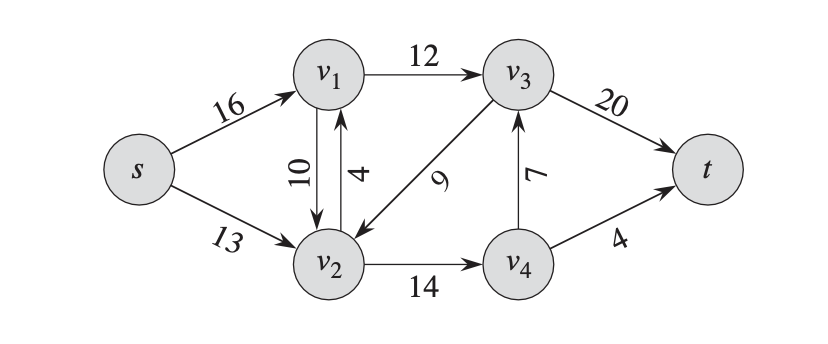
\includegraphics[width=0.5\linewidth]{截屏2024-11-18 下午7.32.25.png}
    \caption{26.1(a)}
    \label{fig:enter-label}
\end{figure}
\section{26.2-3}
%zhigao
\section{26.2-7}
%zhigao
\section{26.2-9}
\section{26.3-2}

\end{document}
